

\section{Besturingssystemen en PWA's}
\label{ch: BesturingssystemenEnPWAs}

Om te weten te komen voor welke toepassingen een PWA gemaakt kan worden en voor welke toepassingen nog steeds een native applicatie nodig is, is het belangrijk om te weten wat de technische mogelijkheden zijn van een PWA. In deze sectie van de literatuurstudie wordt er bekeken welke functies, die beschikbaar zijn voor native applicaties, al dan niet gebruikt kunnen worden door PWA's.

Dit onderzoek werd gevoerd met behulp van de website \href{https://whatwebcando.today/}{whatwebcando.today} en
\href{https://caniuse.com/}{caniuse.com}.

                                 
\href{https://whatwebcando.today/}{whatwebcando.today} is een website die kleine voorbeelden van verschillende technologieën demonstreert. Door deze voorbeelden te testen op verschillende platformen kan er uitgemaakt worden welke technologieën er beschikbaar zijn voor het web, en op welke platformen deze beschikbaar zijn.

\href{https://caniuse.com/}{ caniuse.com} is een website die voor verschillende web-technologieën een overzicht biedt op welke browsers deze technologie gebruikt kan worden en op welke niet. Deze website werd gebruikt om de ondervindingen van de testen die werden uitgevoerd te valideren. 

Een web-API is een API die wordt aangeboden door de browser. Het verschil met web-API's en traditionele API's is dat web-API's lokaal worden aangeboden door de browser en er dus geen internetverbinding nodig is om van deze functionaliteiten te genieten.
\autocite{Mozilla2019c}


Als er meer informatie nodig was over de web API's werd deze gevonden op \href{https://developers.google.com/}{developers.google.com } of op \href{https://developer.mozilla.org/nl/}{MDN web docs}

Er werd gekeken op welke platformen bepaalde functies wel en niet werkten. De volgende platformen werden onderzocht:
\begin{itemize}
   \item Desktop:
   \begin{itemize}
     \item	Microsoft edge versie 80 op Windows 10
     \item	Mozilla firefox versie 73.0 op Windows 10
     \item	Google Chrome versie 79.0 op Windows 10
     \item  Safari (desktop) versie 13.0.5 op een Macbook Pro met macOS Mojave (10.14.6)
   \end{itemize}
\end{itemize}


\begin{itemize}
   \item Mobiel:
   \begin{itemize}
     \item Google Chrome versie 80 op Android 10 op een OnePlus 6
     \item Safari (mobiel) versie 13 op IOS 13 op een IPhone SE 
     
   \end{itemize}
\end{itemize}

De testen werden uitgevoerd op 7 maart 2020.

De website \href{https://whatwebcando.today/}{whatwebcando.today} geeft een overzicht van de functionaliteiten aan de hand van een bepaalde structuur. Deze structuur werd overgenomen en ziet er als volgt uit:
   \begin{itemize}
     \item	Media
     \item	Verbinding
     \item	Toestel kenmerken
     \item	Native gedrag
     \item	Besturingssysteem
     \item	Input
     \item	User experience
     \item	Locatie en positionering
     \item	Scherm en output
   \end{itemize}

\subsection{Onderzoek}

\subsubsection{Media}

\paragraph{Video met audio }

Sommige van de meest populaire mobiele applicaties zijn sterk afhankelijk van camera-functionaliteit. Voorbeelden hiervan zijn Snapchat, Instagram, Messenger, WhatsApp, … 

Bij deze applicaties is het belangrijk dat de camera aan volgende vereisten voldoet:

   \begin{itemize}
     \item	Snel en eenvoudig te gebruiken
     \item	Er moet van camera gewisseld kunnen worden
     \item	Er moet ingezoomd kunnen worden
     \item	De flashlight moet gebruikt kunnen worden
   \end{itemize}

De media capture API \autocite{DzungDTran2012}  maakt het mogelijk om een video die opgenomen wordt met de camera van het toestel te tonen op de webpagina. Deze video kan dan opgeslagen worden in de code en verzonden worden naar een server. 
\autocite{Fransson2017}

De media capture API is ook in staat om aan het toestel te vragen welke camera’s er beschikbaar zijn en dan te verwisselen van camera.
\autocite{Scales2020a}

Ook meer geavanceerde functionaliteiten  zijn beschikbaar. Het gedrag van de zoom en de flashlight kan ook programmatisch bepaald worden.
\autocite{Oberhofer2017} \autocite{Ogundipe2018}


Al de belangrijkste functionaliteiten die een gebruiker verwacht, zijn allemaal aanwezig. Applicaties die afhankelijk zijn van video-opnames kunnen dus geïmplementeerd worden als PWA.

\begin{table}[H]
	\centering
	\begin{tabular}{llllll}
		Edge & Firefox & Chrome & Safari & Android (Chrome) & IOS (Safari) \\
		Ja   & Ja      & Ja     & Ja     & Ja               & Ja          
	\end{tabular}	
	\caption{ondersteuning van de Media Capture API op 7 maart 2020}
\end{table}



\paragraph{Foto's }

Het vastleggen van foto's is ook voor veel populaire applicaties belangrijk. Ook dit is een belangrijke functionaliteit voor sociale media applicaties.

Foto's die gedeeld worden op sociale media moeten vaak van een zo hoog mogelijke kwaliteit zijn. Op native applicaties wordt deze kwaliteit bereikt door volgende eigenschappen: 

 \begin{itemize}
     \item Manuele en automatische focus
     \item Aanpassen van sluitersnelheid
     \item Aanpassen van witbalans
     \item Aanpassen ISO-waarde
     \item Gebruik maken van HDR 
   \end{itemize}

Foto's kunnen ook, net zoals een video, genomen worden aan de hand van de Media capture API. Deze API is echter niet in staat om deze instellingen van de camera aan te passen.

De Image Capture API \autocite{Mandyam2017} is ontwikkeld om meer controle te hebben over de camera. Deze API zorgt ervoor dat instellingen zoals witbalans, temperatuur, exposure, ISO, helderheid, contrast, saturatie, zoom, … programmatisch aangepast kunnen worden.

Deze API heeft standaard geen ondersteuning voor HDR, maar dit kan zelf geïmplementeerd worden aan de hand van ‘third-party-packages’.
\autocite{Bhaumik2019}

\begin{table}[H]
	\centering
	\begin{tabular}{llllll}
		Edge & Firefox & Chrome & Safari & Android (Chrome) & IOS (Safari) \\
		Nee   & Nee      & Ja     & Nee     & Ja               & Nee          
	\end{tabular}	
	\caption{ondersteuning van de Image Capture API op 7 maart 2020}
\end{table}



\paragraph{Geluidopname }



De mediarecorder API, \autocite{CasasSanchez2017} door meerdere browsers aangeboden, is een manier om eenvoudig geluidsfragmenten op te nemen en te importeren in een webapplicatie.

Helaas is er voor Apple-toestellen geen ondersteuning. In de toekomst zal deze functie waarschijnlijk ook beschikbaar worden voor deze toestellen. Dit wordt in de volgende versie van Safari (Safari 14) voor desktop en IOS verwacht. Voor Safari voor IOS bestaat deze functie al maar is het nog een experimentele functie die de gebruiker zelf moet activeren.



\begin{table}[H]
	\centering
	\begin{tabular}{llllll}
		Edge & Firefox & Chrome & Safari & Android (Chrome) & IOS (Safari) \\
		Ja   & Ja      & Ja     & Nee     & Ja               & Nee          
	\end{tabular}	
	\caption{ondersteuning van de Image Capture API op 7 maart 2020}
\end{table}

Gelukkig is er een alternatief voorzien met HTML5-tags. Dit is een methode die voor alle platformen zal werken maar niet op dezelfde manier.

\begin{lstlisting}
<input type="file" accept="audio/*" capture>
\end{lstlisting}

Er wordt gebruik gemaakt van een inputveld waar de gebruiker een bestand kan uploaden. Door het accept attribuut wordt duidelijk gemaakt dat enkel audiofragmenten geüpload mogen worden. Het capture attribuut zorgt ervoor dat waar mogelijk de gebruiker een audiofragment kan opnemen in de default geluidsopname app. Dit fragment wordt dan automatisch geïmporteerd in de webapplicatie. Dit is enkel mogelijk op mobiele toestellen en dus niet in desktopbrowsers.
\autocite{Kinlan2019}

Dit is een goed voorbeeld van progressive enhancement. 



\paragraph{Real-time communicatie }



Bij de meeste populaire communicatieapplicaties zoals WhatsApp, Messenger, Skype, … is videobellen mogelijk. Om dit mogelijk te maken moet er live video en audio gestreamd kunnen worden tussen twee of meer personen.

‘Real-time communication in the web’ of WebRTC \autocite{Jennings2019} is een verzameling van API’s die het verzenden en ontvangen van real-time video en audio mogelijk maakt, zonder afhankelijk te zijn van een gecentraliseerde server. Deze server is echter wel nodig om een connectie tot stand te brengen. Eens deze connectie er is, is er een peer-to-peer verbinding.

\begin{table}[H]
	\centering
	\begin{tabular}{llllll}
		Edge & Firefox & Chrome & Safari & Android (Chrome) & IOS (Safari) \\
		Ja   & Ja      & Ja     & Ja     & Ja               & ja          
	\end{tabular}	
	\caption{ondersteuning van WebRTC op 7 maart 2020}
\end{table}




\paragraph{Casting}

Applicaties die media tonen aan de gebruiker kunnen deze casten naar tv-toestel. Dit gebeurt bij Apple toestellen aan de hand van Airplay en bij Android toestellen aan de hand van google cast.


YouTube is een applicatie die hier gebruik van maakt. Als er een video bekeken wordt, zal de gebruiker een optie krijgen om deze te tonen op een tv.


Op Apple toestellen kan een PWA nu ook AirPlay implementeren. 
\autocite{Apple2020a}


De Chrome Sender API \autocite{Developers2020b} zorgt ervoor dat alle modern toestellen media kunnen delen op een tv of ander scherm die dit ondersteunt.

\begin{table}[H]
	\centering
	\begin{tabular}{llllll}
		Edge & Firefox & Chrome & Safari & Android (Chrome) & IOS (Safari) \\
		Nee   & Nee      & Nee     & Ja     & Nee               & Ja          
	\end{tabular}	
	\caption{ondersteuning Apple AirPlay op 7 maart 2020}
\end{table}
\begin{table}[H]
	\centering
	\begin{tabular}{llllll}
		Edge & Firefox & Chrome & Safari & Android (Chrome) & IOS (Safari) \\
		Ja   & Ja      & Ja     & Ja     & Ja               & ja          
	\end{tabular}	
	\caption{ondersteuning van Chrome Sender API op 7 maart 2020}
\end{table}




\paragraph{Media-controle in de notificatie }


Als een native applicatie media afspeelt op een mobiel toestel, kan deze applicatie bestuurd worden vanuit de notificatie. De afgespeelde media zal ook niet stoppen als een gebruiker de applicatie verlaat

Een voorbeeld hiervan is Spotify, in de notificatie van Spotify kan de gebruiker volgende acties uitvoeren.
 \begin{itemize}
   \item	Informatie bekijken over het nummer
   \item	Naar het volgende nummer gaan
   \item	Het nummer pauzeren
   \item	Het nummer toevoegen aan “mijn favorieten”
   \item	De vooruitgang van het nummer zien en aanpassen
\end{itemize}
De Media Session API \autocite{Beaufort2019} zorgt ervoor dat als er media afgespeeld wordt op een website, en de browser wordt gesloten, de media niet zal stoppen met afspelen.

Deze API zorgt er ook voor dat er een notificatie komt waar de gebruiker controle heeft over de afgespeelde media. 

Het voorbeeld van Spotify kan dus volledig geïmplementeerd worden als PWA.

\begin{table}[H]
	\centering
	\begin{tabular}{llllll}
		Edge & Firefox & Chrome & Safari & Android (Chrome) & IOS (Safari) \\
		Ja   & Ja      & Ja     & Ja     & Ja               & ja          
	\end{tabular}	
	\caption{ondersteuning van Media Session API op 7 maart 2020}
\end{table}



\subsubsection{Connectie met andere apparaten}



\paragraph{Bluetooth }

Native applicaties kunnen een verbinding maken met bluetooth-toestellen. Eens er een verbinding is, kan er informatie uitgewisseld worden tussen de toestellen. Een voorbeeld van een applicatie die hier gebruik van maakt is de ‘Sony Headphones’ app. Aan de hand van deze app kan er verbinding gemaakt worden met een koptelefoon en kunnen de instellingen van de koptelefoon aangepast worden.

Met de Web Bluetooth API \autocite{Grant2020} kan er vanuit de browser verbinding gemaakt worden met bluetooth-toestellen. De web API heeft zowel schrijf- als leesrechten bij externe toestellen. 

Er kan dus geconcludeerd worden dat de Web Bluetooth API kan gebruikt worden voor applicaties die gebruik moeten maken van bluetooth-toestellen.
\autocite{Beaufort2019a}

\begin{table}[H]
	\centering
	\begin{tabular}{llllll}
		Edge & Firefox & Chrome & Safari & Android (Chrome) & IOS (Safari) \\
		Ja   & Nee      & Ja     & Nee     & Ja               & Nee          
	\end{tabular}	
	\caption{ondersteuning van Web Bluetooth API op 7 maart 2020}
\end{table}



\paragraph{USB}

Verkopers van toestellen met USB kunnen nu gebruik maken van de Web USB API, \autocite{Rockot2020}. Bij het verbinden van een USB-toestel kan er automatisch een website geopend worden waarmee het toestel kan interageren.
 
Dit kan interessant zijn voor toestellen die een eenmalige set-up nodig hebben. Met deze technologie kan vermeden worden dat er overbodige software moet geïnstalleerd worden op het toestel van de gebruiker. 

Dit is echter enkel mogelijk met een beperkt aantal browsers en er moet een HTTPS-verbinding zijn.
\autocite{Beaufort2019b}

\begin{table}[H]
	\centering
	\begin{tabular}{llllll}
		Edge & Firefox & Chrome & Safari & Android (Chrome) & IOS (Safari) \\
		Ja   & Nee      & Ja     & Nee     & Ja               & Nee          
	\end{tabular}	
	\caption{ondersteuning van Web USB API op 7 maart 2020}
\end{table}


\paragraph{NFC}

Near field communication of NFC is een technologie om een kleine hoeveelheid informatie uit te wisselen over een kleine afstand (Maximum 20cm). NFC wordt gebruikt om draadloze betalingen uit te voeren met een betaalkaart of met een smartphone. 
\autocite{Paus2007}

\begin{table}[H]
	\centering
	\begin{tabular}{llllll}
		Edge & Firefox & Chrome & Safari & Android (Chrome) & IOS (Safari) \\
		Nee   & Nee      &  Nee     & Nee     & Nee               & Nee          
	\end{tabular}	
	\caption{ondersteuning van Web NFC API op 7 maart 2020}
\end{table}

Dit is een functie met veel mogelijkheden die helaas niet beschikbaar is voor webapplicaties.
Er bestaat echter wel een API om gebruik te kunnen maken van NFC \autocite{RohdeChristiansen2020}, maar de Web NFC API is een experimentele API. Dit betekent dat de eindgebruiker dit nog niet kan gebruiken.



\subsubsection{Toestelkenmerken}


\paragraph{Netwerkinformatie}

De Network information API \autocite{Lamouri2014} voorziet informatie over het type netwerkverbinding die de gebruiker momenteel bezit. Deze informatie bevat het connectietype (2g, 3g, 4g) en wat de maximale downloadsnelheid is van deze verbinding.

\begin{table}[H]
	\centering
	\begin{tabular}{llllll}
		Edge & Firefox & Chrome & Safari & Android (Chrome) & IOS (Safari) \\
		Nee   & Nee      &  Ja     & Nee     & Ja               & Nee          
	\end{tabular}	
	\caption{ondersteuning van Network information API op 7 maart 2020}
\end{table}

\paragraph{Online status}

Dit is een eenvoudige eigenschap die kan opgeroepen worden op het navigator object. Deze eigenschap bevat een booleaanse waarde die “waar” zal zijn als de gebruiker een connectie heeft met het internet. 

Dit is een belangrijke eigenschap bij applicaties die real-time data gebruiken. Als de internetconnectie van de gebuiker wegvalt kan er een melding  getoond worden. Op deze manier weet de gebruiker dat de data mogelijks niet up-to-date is.
\begin{table}[H]
	\centering
	\begin{tabular}{llllll}
		Edge & Firefox & Chrome & Safari & Android (Chrome) & IOS (Safari) \\
		Ja   & Ja      &  Ja     & Ja     & Ja               & Ja          
	\end{tabular}	
	\caption{ondersteuning online status op 7 maart 2020}
\end{table}

\paragraph{Vibratiemotor }

De Vibration API \autocite{Kostionen2018} zorgt ervoor dat de vibratiemotor kan aangesproken worden vanuit de webapplicatie.

\begin{table}[H]
	\begin{tabular}{llllll}
		Edge & Firefox & Chrome & Safari & Android (Chrome) & IOS (Safari) \\
		Ja   & Ja      &  Ja     & Nee     & Ja               & Nee          
	\end{tabular}	
	\caption{ondersteuning vibratiemotor  op 7 maart 2020}
\end{table}


\paragraph{Batterijstatus}

Aan de hand van de Battery Status API \autocite{Kostiainen2016} kan er informatie over de batterij van het toestel verkregen worden.

Volgende informatie kan verkregen worden:
 \begin{itemize}
	\item	Aan het opladen
	\item	Batterijpercentage
	\item	Bij opladen, tijd tot volladen
	\item	Bij niet opladen, tijd tot batterij leeg
\end{itemize}

Aan de hand van deze API kunnen er ook acties uitgevoerd worden op basis van het veranderen van de toestand van de batterij. Er kan bijvoorbeeld een functie uitgevoerd worden als de gebruiker zijn toestel met een energiebron verbindt.

\begin{table}[H]
	\centering
	\begin{tabular}{llllll}
		Edge & Firefox & Chrome & Safari & Android (Chrome) & IOS (Safari) \\
		Ja   & Nee      &  Ja     & Nee     & Ja               & Nee          
	\end{tabular}	
	\caption{ondersteuning batterijstatus op 7 maart 2020 }
\end{table}

\paragraph{Toestelgeheugen}
de Device Memory API \autocite{Panicker2018} geeft informatie over het RAM-geheugen van het toestel van de gebruiker. Dit kan interessant zijn voor het laden van een eventuele lichtere versie van een website voor minder capabele toestellen.

\begin{table}[H]
	\centering
	\begin{tabular}{llllll}
		Edge & Firefox & Chrome & Safari & Android (Chrome) & IOS (Safari) \\
		Ja   & Nee      &  Ja     & Nee     & Ja               & Nee          
	\end{tabular}	
	\caption{ondersteuning toestelgeheugen op 7 maart 2020}
\end{table}



\subsubsection{Native gedrag}

\paragraph{Lokale notificaties}
Bij native applicaties kan een bepaalde actie binnen de app resulteren in een notificatie. Veel gezondheids-tracking applicaties maken hier gebruik van. Een gebruiker zal bijvoorbeeld een melding krijgen als een vooropgesteld aantal stappen op een dag is bereikt.

Lokale notificaties zijn beschikbaar via de Notifications API \autocite{Gregg2015}. Lokale notificaties zijn notificaties die geen internet of server nodig hebben. Deze kunnen gepland worden bij het laden van de website. Ze worden dus lokaal geactiveerd.

Meer informatie over notificaties kan gevonden worden in het hoofdstuk \ref{ch: Functionaliteiten die een serivce worker mogelijk maakt}.

Dankzij persistent local notifications en zijn service worker kan het voorbeeld van de fitness-tracking applicatie ook geïmplementeerd worden als PWA.

\begin{table}[H]
	\centering
	\begin{tabular}{llllll}
		Edge & Firefox & Chrome & Safari & Android (Chrome) & IOS (Safari) \\
		Ja   & Nee      &  Ja     & Nee     & Ja               & Nee          
	\end{tabular}	
	\caption{ondersteuning lokale notificaties op 7 maart 2020}
\end{table}

\paragraph{Push notificaties}

Native applicaties kunnen genieten van notificaties die niet geactiveerd worden vanop het toestel zelf. Een voorbeeld hiervan is een sport-applicatie die een melding geeft als de gebruiker zijn favoriete voetbalploeg een doelpunt heeft gemaakt.

Push notificaties zijn notificaties die verstuurd worden vanop een server. Door gebruik te maken van de Push API \autocite{Sullivan2020} om notificaties te ontvangen en de Notification API om notificaties op het scherm te tonen, kan een PWA push notificaties implementeren. 

Meer informatie over notificaties kan gevonden worden in het hoofdstuk \ref{ch: Functionaliteiten die een serivce worker mogelijk maakt}.

Door deze functionaliteiten kan het voorbeeld van een sportapplicatie ook geïmplementeerd worden als PWA.

\begin{table}[H]
	\centering
	\begin{tabular}{llllll}
		Edge & Firefox & Chrome & Safari & Android (Chrome) & IOS (Safari) \\
		Ja   & Ja      &  Ja     & Nee     & Ja               & Nee          
	\end{tabular}	
	\caption{ondersteuning push notificaties op 7 maart 2020}
\end{table}



\paragraph{A2HS}


 Door het toevoegen van een web app manifest kan je de browser duidelijk maken hoe een applicatie er moet uitzien als het toegevoegd wordt aan het startscherm. De PWA zal er dan op het startscherm gelijk uitzien als een native applicatie.
	Meer informatie over notificaties kan gevonden worden in het hoofdstuk \ref{ch: Functionaliteiten die een serivce worker mogelijk maakt}..


\begin{table}[H]
	\centering
	\begin{tabular}{llllll}
		Edge & Firefox & Chrome & Safari & Android (Chrome) & IOS (Safari) \\
		Ja   & Ja      &  Ja     & Nee     & Ja               & Nee          
	\end{tabular}	
	\caption{ondersteuning A2HS op 7 maart 2020 }
\end{table}


\paragraph{Badges}

Als een native applicatie een melding heeft ontvangen zal er een indicatie staan naast het icoontje op het startscherm. Dit kan nu ook geïmplementeerd worden voor geïnstalleerde PWA's aan de hand van de Badging API. \autocite{LePage2020a}

Op sommige applicatie zal hier een indicatie staan van het aantal meldingen.
\begin{table}[H]
	\centering
	\begin{tabular}{llllll}
		Edge & Firefox & Chrome & Safari & Android (Chrome) & IOS (Safari) \\
		Ja   & Onbekend      &  Ja     & Nee     & Ja               & Nee          
	\end{tabular}	
	\caption{ondersteuning Badging API op 7 maart 2020}
\end{table}

\paragraph{Voorgrond-detectie }

Native applicaties kunnen detecteren als een applicatie op de voorgrond wordt gebruikt. YouTube maakt hier gebruik van om zeker te zijn dat de gebruiker de applicatie actief gebruikt op het moment dat een advertentie getoond wordt.

Met de Page Visibility Detection API \autocite{Grigorik2017} kan gedetecteerd worden of een applicatie in de voorgrond gebruikt wordt of niet. 

Aan de hand van deze applicatie kan het gedrag van de applicatie aangepast worden als de gebruiker de applicatie niet meer in de voorgrond gebruikt.

\begin{table}[H]
	\centering
	\begin{tabular}{llllll}
		Edge & Firefox & Chrome & Safari & Android (Chrome) & IOS (Safari) \\
		Ja   & Ja      &  Ja     & Ja     & Ja               & Ja          
	\end{tabular}	
	\caption{ondersteuning voorgrond detectie op 7 maart 2020}
\end{table}


\paragraph{Toestemmingen}

Om gebruik te maken van hardware functies van een toestel is vaak, om privacy redenen, de toestemming van de gebruiker nodig. Hiervoor is de Permissions API \autocite{Caceres2017} ontwikkeld. Er kan toestemming gevraagd worden op een gelijkaardige manier voor verschillende functies.

Functies waarvoor toestemming gevraagd kan worden:
 \begin{itemize}
	\item	Locatie
	\item	Notificaties
	\item	Push-notificaties
	\item	Midi (musical instrument digital interface)
	\item	Klembord
	\item	Camera
	\item	Microfoon
	\item	Achtergrondsynchronisatie
	\item	Lichtsensor
	\item	Versnellingsmeter
	\item	Gyroscoop
	\item	Magneetsensor
	\item	Betalingen
\end{itemize}

	\begin{table}[H]
		\centering
		\begin{tabular}{llllll}
			Edge & Firefox & Chrome & Safari & Android (Chrome) & IOS (Safari) \\
			Ja   & Ja      &  Ja     & nee     & Ja               & nee          
		\end{tabular}	
		\caption{ondersteuning Permissions API op 7 maart 2020}
	\end{table}
	

\subsubsection{Besturingssysteem}
\paragraph{offline opslage}
Native applicaties kunnen nog steeds gebruikt worden als er geen internetverbinding is. Toepassingen die geen netwerkverzoeken doen zijn dus nog volledig operationeel zonder internetverbinding. 

Er zijn verschillende technologieën om data offline op te slaan. 

 \begin{itemize}
	\item	Web storage
	\item	IndexedDB
	\item	Cache API
	\item	Storage API
\end{itemize}

	\subparagraph{Web storage}
	De meest eenvoudige manier om data op te slaan. Er kunnen key-value paren opgeslagen worden in het localStorage of in het sessionStorage. 
	\autocite{Hickson2016}
	
	\begin{table}[H]
		\centering
		\begin{tabular}{llllll}
			Edge & Firefox & Chrome & Safari & Android (Chrome) & IOS (Safari) \\
			Ja   & Ja      &  Ja     & Ja     & Ja               & Ja          
		\end{tabular}	
		\caption{ondersteuning web storrage op 7 maart 2020}
	\end{table}
	
	
	
	\subparagraph{IndexedDB}
	Een API voor het opslaan van grote hoeveelheden gestructureerde data op het toestel van de eindgebruiker. De data kan snel gelezen worden omdat er indexen gebruikt worden. 
	\autocite{Alabbas2018}
	
	\begin{table}[H]
		\centering
			\begin{tabular}{llllll}
				Edge & Firefox & Chrome & Safari & Android (Chrome) & IOS (Safari) \\
				Ja   & Ja      &  Ja     & Ja     & Ja               & Ja          
			\end{tabular}	
			\caption{ondersteuning IndexedDB op 7 maart 2020}
	\end{table}
	
	
	\subparagraph{Cache API}
	Deze API is gespecialiseerd in het opslaan van netwerkverzoeken. Dit is heel handig in samenwerking met een serviceworker. API-calls kunnen opgeslagen worden voor offline gebruik.
	\autocite{vanKesteren2008}
	
	\begin{table}[H]
		\centering
			\begin{tabular}{llllll}
				Edge & Firefox & Chrome & Safari & Android (Chrome) & IOS (Safari) \\
				Ja   & Ja      &  Ja     & Ja     & Ja               & Nee          
			\end{tabular}	
			\caption{ondersteuning Cache API op 7 maart 2020}
	\end{table}
	
	
	\subparagraph{Storage API}
	Data die is opgeslagen in een van vorige technologieën kan eenvoudig verwijderd worden door de browser. Met de storage API kan data opgeslagen worden op het systeem voor een langere periode .
	\autocite{Mozilla2020b}
	
	\begin{table}[H]
		\centering
		\begin{tabular}{llllll}
			Edge & Firefox & Chrome & Safari & Android (Chrome) & IOS (Safari) \\
			Ja   & Ja      &  Ja     & Ja     & Ja               & Nee          
		\end{tabular}	
		\caption{ondersteuning Storage API op 7 maart 2020}
	\end{table}
	
	
	
Door gebruik te maken van deze verschillende API’s kan er ook een offline ervaring aangeboden worden aan de gebruiker. 
	
\paragraph{Bestandentoegang}

Native applicaties hebben toegang tot het volledige bestandssysteem van het toestel. Er kunnen bestaande bestanden gelezen en aangepast worden. Er kunnen ook nieuwe bestanden aangemaakt en opgeslagen worden.

Door gebruik te maken van de File API \autocite{Kruisselbrink2019} heeft een webapplicatie ook toegang tot het bestandssysteem. Bestanden kunnen gelezen worden en metadata over deze bestanden kan verkregen worden.

Een webapplicatie heeft echter enkel leesrechten op deze bestanden. Er kunnen dus geen bestanden geschreven of aangepast worden.

Dit betekent dus dat bepaalde toepassingen die hier gebruik van maken nog steeds een native applicatie nodig hebben.

\begin{table}[H]
	\centering
	\begin{tabular}{llllll}
		Edge & Firefox & Chrome & Safari & Android (Chrome) & IOS (Safari) \\
		Ja   & Ja      &  Ja     & Nee     & Ja               & Nee          
	\end{tabular}	
	\caption{ondersteuning File API op 7 maart 2020}
\end{table}	


\paragraph{Contacten}
Bepaalde native applicaties hebben toegang nodig tot de contacten van de gebruiker. Een voorbeeld hiervan is WhatsApp. Deze importeert de contacten van het toestel in de applicatie.

De contacten die opgeslagen staan op het systeem van de gebruiker kunnen geïmporteerd worden in een webapplicatie met de Contacts API \autocite{Tibbett2014}.

In theorie zouden PWA's hier dus gebruik kunnen van maken maar de ondersteuning is heel beperkt. Het is dus niet aangeraden om een webapplicatie te ontwikkelen die afhankelijk is van de contacten van een gebruiker.

\begin{table}[H]
	\centering
	\begin{tabular}{llllll}
		Edge & Firefox & Chrome & Safari & Android (Chrome) & IOS (Safari) \\
		Nee   & Nee      &  Nee     & Nee     & Beperkt *               & Nee          
	\end{tabular}	
	\caption{ondersteuning Contacts API op 7 maart 2020}{ * Op het moment van schrijven is dit een nieuwe en experimentele functie die enkel werkt op 
	Android 10. Verdere ondersteuning is nog onbekend.}
\end{table}	


\paragraph{Sms}
Native Applicaties kunnen binnenkomende sms-berichten lezen. Dit wordt vaak gebruikt om de authenticatie van een gebruiker sneller te laten verlopen. Een voorbeeld van deze use-case kan bij de applicatie van het betalingsplatform PayPal gevonden worden. Als een gebruiker zich registreert, zal zijn telefoonnummer gecontroleerd worden door er een sms naar dit nummer te sturen met een code. PayPal zal zien dat er een sms binnenkomt en zal automatisch de code uit dit bericht halen. Op deze manier hoeft de gebruiker de app niet te verlaten.

Native applicaties kunnen niet enkel sms’en lezen, ze kunnen er ook schrijven. Dit betekent dus dat elke ontwikkelaar een sms-client applicatie kan maken.

Met de SMS-receiver API \autocite{Fullea2015} kan er gekeken worden naar inkomende sms’en. Het voorbeeld van de PayPal applicatie kan dus ook geïmplementeerd worden als PWA. PWA's hebben echter enkel toegang tot binnenkomende sms’en. 

Het voorbeeld van PayPal kan ook geïmplementeerd worden aan de hand van een PWA. Applicaties die ook sms-berichten moeten versturen kunnen niet ontwikkeld worden als PWA.

\begin{table}[H]
	\centering
	\begin{tabular}{llllll}
		Edge & Firefox & Chrome & Safari & Android (Chrome) & IOS (Safari) \\
		Nee   & Nee      &  Nee     & Nee     & Beperkt *             & Nee          
	\end{tabular}	
	\caption{ondersteuning Messaging API op 7 maart 2020}{* Op het moment van schrijven is dit een nieuwe en experimentele functie die enkel werkt op 
		Android 10. Verdere ondersteuning is nog onbekend.}
\end{table}	



\paragraph{Taakplanning}
De Task Sheduler API \autocite{Kulkarni2015} kan ervoor zorgen dat taken zoals alarmen, herinneringen en gelijkaardige taken kunnen ingepland worden in het systeem. Deze API is slechts een voorstel en heeft dus nog geen ondersteuning.

Een applicatie schrijven die het alarm van een smartphone in de ochtend laat afgaan, of een activiteit in jouw agenda plaatst, is dus niet mogelijk met een PWA. Dit zijn toepassingen die wel mogelijk zijn met native applicaties.

\begin{table}[H]
	\centering
	\begin{tabular}{llllll}
		Edge & Firefox & Chrome & Safari & Android (Chrome) & IOS (Safari) \\
		Nee   & Nee      &  Nee     & Nee     & Nee               & Nee          
	\end{tabular}	
	\caption{ondersteuning Task Sheduler API op 7 maart 2020}
\end{table}	



\subsubsection{Input}

\paragraph{Touch gebaren}

Native applicaties hebben een verwachtingspatroon ontwikkeld bij de gebruiker. Voorbeelden hiervan zijn:

 \begin{itemize}
	\item	Swipe van links opent het menu
	\item	Knijpen om in te zoomen
\end{itemize}

HTML5 voegt aan de reeds bestaande input methodes nu ook touch-controls toe. Dit is belangrijk om een applicatie intuïtief te laten werken. Het is logisch dat Safari op desktop dit niet ondersteunt aangezien Safari enkel kan gedownload worden op Mac-toestellen en geen enkel Mac-toestel een touchscreen heeft.

Deze gebaren kunnen nu ook gebruikt worden in een PWA. Dit zorgt ervoor dat een geïnstalleerde PWA meer zal aanvoelen als een native applicatie.

\begin{table}[H]
	\centering
	\begin{tabular}{llllll}
		Edge & Firefox & Chrome & Safari & Android (Chrome) & IOS (Safari) \\
		Ja   & Ja      &  Ja     & Ja     & ja               & Ja          
	\end{tabular}	
	\caption{ondersteuning touch gebaren op 7 maart 2020}
\end{table}	

\paragraph{Klembord toegang}
De Clipboard API \autocite{Kacmarcik2010} geeft een ontwikkelaar de mogelijkheid om te interageren met het klembord. Er kunnen zowel items van het klembord gelezen worden als dat er items kunnen geschreven worden naar het klembord.

Er worden ook methodes voorzien voor het reageren op de actie waarbij een gebruiker zelf iets kopieert of plakt. 

\begin{table}[H]
	\centering
	\begin{tabular}{llllll}
		Edge & Firefox & Chrome & Safari & Android (Chrome) & IOS (Safari) \\
		Ja   & Ja      &  Ja     & Ja     & ja               & Ja          
	\end{tabular}	
	\caption{ondersteuning Clipboard API op 7 maart 2020}
\end{table}	


\subsubsection{User experience}

\paragraph{Offline gebruik}
Door het gebruik van serviceworkers kan een website offline gebruikt worden. Deze website moet eerst bezocht worden als de gebruiker online is. De geladen pagina’s en andere items zoals foto’s kunnen opgeslagen worden voor offline gebruik.

\begin{table}[H]
	\begin{tabular}{llllll}
		Edge & Firefox & Chrome & Safari & Android (Chrome) & IOS (Safari) \\
		Ja   & Ja      &  Ja     & Ja     & ja               & Ja          
	\end{tabular}	
	\caption{ondersteuning offline gebruik op 7 maart 2020}
\end{table}	



\paragraph{Achtergrondsynchronisatie }

Een actie kan van start gaan als de gebruiker een trage verbinding heeft of als hij offline is. Achtergrondsynchronisatie zal ervoor zorgen dat deze actie uitgevoerd wordt vanaf dat er een stabiele internetconnectie is, zelfs al is de applicatie reeds gesloten.

Meer info over achtergrondsynchronisatie kan gevonden worden in het hoofdstuk “Functionaliteiten die een serivce worker mogelijk maakt”.


\begin{table}[H]
	\centering
	\begin{tabular}{llllll}
		Edge & Firefox & Chrome & Safari & Android (Chrome) & IOS (Safari) \\
		Ja   & Ja      &  Ja     & Ja     & ja               & Ja          
	\end{tabular}	
	\caption{ondersteuning achtergrondsynchronisatie op 7 maart 2020}
\end{table}


\paragraph{Inter-app communicatie}
Native applicaties kunnen gebruik maken van deep-linking, dit is een concept waarbij er in een app een link kan staan naar een specifieke pagina op een andere app.

De Web Share API \autocite{Giuca2019} en de Web Share Target API \autocite{Williger2019} zorgen ervoor dat links van websites kunnen geopend worden in native applicaties. 

De web Share API moet gebruikt worden in de applicatie die een link heeft naar een andere applicatie.

De web Share Target API moet gebruikt worden in de applicatie waarnaar gerefereerd wordt. Deze zal ervoor zorgen dat de gebruiker uiteindelijk op de juiste pagina terecht komt.

\begin{table}[H]
	\centering
	\begin{tabular}{llllll}
		Edge & Firefox & Chrome & Safari & Android (Chrome) & IOS (Safari) \\
		Nee   & Nee      &  Nee     & Nee     & ja               & Ja          
	\end{tabular}	
	\caption{ondersteuning Web Share API en Web Share Target API op 7 maart 2020}
\end{table}



\paragraph{Betalingen}
Aan de hand van de Payment Request API \autocite{Denicola2019} kan heel snel, zonder de website te verlaten, een betaling uitgevoerd worden. Bij Apple-toestellen zal dit gebeuren via Apple-pay. 

\begin{table}[H]
	\centering
	\begin{tabular}{llllll}
		Edge & Firefox & Chrome & Safari & Android (Chrome) & IOS (Safari) \\
		Ja   & Nee      &  Ja     & Ja     & ja               & Ja          
	\end{tabular}	
	\caption{ondersteuning Payment Request API op 7 maart 2020}
\end{table}


\paragraph{Credentials}
De Credential Management API \autocite{West2019} levert methodes voor het ophalen en opslaan van de credentials van een gebruiker. Op deze manier kan de gebruiker eenvoudiger en veiliger aanmelden op een platform.

\begin{table}[H]
	\begin{tabular}{llllll}
		Edge & Firefox & Chrome & Safari & Android (Chrome) & IOS (Safari) \\
		Ja   & Nee      &  Ja     & Nee     & ja               & Nee          
	\end{tabular}	
	\caption{ondersteuning Credential Management API op 7 maart 2020}
\end{table}

\subsubsection{Locatie en positionering}

\paragraph{Geolocatie}
De Geolocation API \autocite{Popescu2018} zorgt ervoor dat een applicatie toegang heeft tot de locatie van een toestel. Dat wordt gedaan op basis van de gps-sensor of op basis van het netwerk. 

Zowel de lengtegraad als de breedtegraat kunnen opgevraagd worden, deze twee coördinaten vormen de locatie van de gebruiker.


De Geolocation API voorziet een methode "watchPosition". Elke keer dat de locatie van een gebruiker verandert, zal deze methode een functie aanroepen. Op deze manier kan de locatie van een gebruiker gevolgd worden.

Navigatie-applicaties zoals Google Maps of Waze kunnen dus ook geïmplementeerd worden als PWA.

\begin{table}[H]
	\centering
	\begin{tabular}{llllll}
		Edge & Firefox & Chrome & Safari & Android (Chrome) & IOS (Safari) \\
		Ja   & Ja      &  Ja     & Ja     & ja               & Ja          
	\end{tabular}	
	\caption{ondersteuning Geolocation API op 7 maart 2020}
\end{table}


\paragraph{Geofencing}
Geofencing is een technologie waarbij er een geografische zone wordt ingesteld. Als de gebruiker in deze zone komt, wordt er automatisch een actie uitgevoerd. 

Er was een voorstel om deze API \autocite{Kruisselbrink2017} uit te werken voor het web, maar op het moment van schrijven heeft geen enkele browser dit geïmplementeerd. Dit is eenfunctie die enkel beschikbaar is voor native IOS en Android-applicaties.

\begin{table}[H]
	\centering
	\begin{tabular}{llllll}
		Edge & Firefox & Chrome & Safari & Android (Chrome) & IOS (Safari) \\
		Nee   & Nee      &  Nee     & Nee     & Nee               & Nee          
	\end{tabular}	
	\caption{ondersteuning Geofencing API op 7 maart 2020}
\end{table}

\paragraph{Toesteloriëntatie }

Native applicaties en meer specifiek, mobiele games maken vaak gebruik van de toesteloriëntatie als input methode. Dit wordt bijvoorbeeld gebruikt bij racegames om een stuur te simuleren.

De Device Orientation API \autocite{Tibbett2019} levert methodes voor het detecteren van de oriëntatie van het toestel. Er zijn drie eigenschappen die de oriëntatie bepalen:


 \begin{itemize}
	\item	Alpha:  Dit is de richting naar waar het toestel gericht is.
	\item	Beta:  Dit is het aantal graden dat het toestel voorwaarts of achterwaarts gekanteld is.
	\item   Gamma: Dit is het aantal graden dat het toestel naar links of naar rechts gekanteld is.
\end{itemize}


De toesteloriëntatie kan, net zoals bij native applicaties, gebruikt worden als een input-methode voor applicaties. Dit wordt vaak gebruikt bij games.

Deze API levert ook methodes die website in een bepaalde oriëntatie forceren.

Niet elk toestel heeft deze sensoren. Als ze aanwezig zijn, worden ze ondersteund in volgende browsers. Deze API is vooral gericht naar mobiele toestellen. 

\begin{table}[H]
	\centering
	\begin{tabular}{llllll}
		Edge & Firefox & Chrome & Safari & Android (Chrome) & IOS (Safari) \\
		Ja   & Ja      &  Ja   & Nee     & Ja               & Ja          
	\end{tabular}	
	\caption{ondersteuning Device Orientation API op 7 maart 2020}
\end{table}

\paragraph{Toestelbeweging}
De Generic Sensor API \autocite{Waldroon2019} is een verzameling van API’s voor het gebruiken van verschillende sensoren van het toestel.

	\subparagraph{DeviceMotionEvent }
	Levert informatie over de snelheid waarmee een toestel zijn oriëntatie en positie verandert.
	
	\begin{table}[H]
		\centering
		\begin{tabular}{llllll}
			Edge & Firefox & Chrome & Safari & Android (Chrome) & IOS (Safari) \\
			Ja   & Ja      &  Ja   & Nee     & Ja               & Ja          
		\end{tabular}	
		\caption{ondersteuning	DeviceMotionEvent  }
	\end{table} 
	
	
	\subparagraph{Accelerometer  }
		Levert informatie over de snelheid waarbij het toestel zich beweegt in een ruimte. De API levert zowel X-, Y- als Z-coördinaten
		
		\begin{table}[H]
			\centering
			\begin{tabular}{llllll}
				Edge & Firefox & Chrome & Safari & Android (Chrome) & IOS (Safari) \\
				Ja   & Nee      &  Ja   & Nee     & Ja               & Nee          
			\end{tabular}	
			\caption{ondersteuning	Accelerometer   }
		\end{table}
		
		
		
	\subparagraph{Gyroscope  }
		Levert informatie over de snelheid waarmee een toestel aan het roteren is. 
			
		\begin{table}[H]
			\centering
			\begin{tabular}{llllll}
				Edge & Firefox & Chrome & Safari & Android (Chrome) & IOS (Safari) \\
				Ja   & Nee      &  Ja   & Nee     & Ja               & Nee          
			\end{tabular}	
			\caption{ondersteuning Gyroscope op 7 maart 2020 }
		\end{table}
			
	\subparagraph{Magnetometer }
			Meet het magnetische veld rond het toestel. 
			
		\begin{table}[H]
			\centering
			\begin{tabular}{llllll}
				Edge & Firefox & Chrome & Safari & Android (Chrome) & IOS (Safari) \\
				Nee   & Nee      &  Ja   & Nee     & Nee               & Nee          
			\end{tabular}	
			\caption{ondersteuning Magnetometer op 7 maart 2020 }
		\end{table}
			
			
	\subparagraph{Lineaire accelerometer}
		Levert informatie over de snelheid waarmee een toestel beweegt, maar dit zonder de impact van de zwaartekracht.
			
		\begin{table}[H]
			\centering
			\begin{tabular}{llllll}
				Edge & Firefox & Chrome & Safari & Android (Chrome) & IOS (Safari) \\
				Ja   & Nee      &  Ja   & Nee     & Ja               & Nee          
			\end{tabular}	
			\caption{ondersteuning Lineaire accelerometer  op 7 maart 2020 }
		\end{table}
		
			
\paragraph{Nabijheid-sensoren }
De Proximity API \autocite{Kostiainen2019} geeft informatie over de afstand tussen het toestel en een object. Deze sensor wordt gebruikt om het scherm uit te zetten als een persoon aan het bellen is.

\begin{table}[H]
	\centering
	\begin{tabular}{llllll}
		Edge & Firefox & Chrome & Safari & Android (Chrome) & IOS (Safari) \\
		Nee   & Ja      &  Nee   & Nee     & Nee               & Nee          
	\end{tabular}	
	\caption{ondersteuning  Proximity API op 7 maart 2020 }
\end{table}



\subsubsection{Scherm en output}
\paragraph{Virtual en augmented reality }
De webXR Device API \autocite{Jones2019} zorgt voor een interface voor het verbinden van een virtual reality toestel met de browser. De sensoren van het toestel kunnen gebruikt worden om het canvas-element te laden in het VR-toestel.

De oudere webVR API levert gelijkaardige methodes maar is beter ondersteund.

\begin{table}[H]
	\centering
	\begin{tabular}{llllll}
		Edge & Firefox & Chrome & Safari & Android (Chrome) & IOS (Safari) \\
		Ja (webXR)  & 	Ja (webVR)  &  	Ja (webVR + webXR  & Nee  & Ja (webVR + webXR) & Nee Nee          
	\end{tabular}	
	\caption{ondersteuning  WebVR en WebXR op 7 maart 2020 }
\end{table}\

\paragraph{Fullscreen }
De Fullscreen API \autocite{Kesteren2014} geeft een aantal methodes die ervoor zorgen dat de browser-elementen verwijderd worden. Dit laat een website meer aanvoelen als een native applicatie.

Er worden twee methodes voorzien: een voor in fullscreen mode te gaan en een om deze te verlaten.

\begin{table}[H]
	\begin{tabular}{llllll}
		Edge & Firefox & Chrome & Safari & Android (Chrome) & IOS (Safari) \\
		Ja   & Ja      &  Ja   & Ja     & Ja               & Nee          
	\end{tabular}	
	\caption{ondersteuning  Fullscreen API op 7 maart 2020 }
\end{table}


\paragraph{Wake lock }
eel toestellen gaan het scherm dimmen na een bepaalde tijd van inactiviteit. Dit kan onhandig zijn voor bepaalde applicaties zoals een gps. Met de Wake Lock API \autocite{Bogdanovich2017} kan het automatisch dimmen van het scherm tegengegaan worden.

\begin{table}[H]
	\centering
	\begin{tabular}{llllll}
		Edge & Firefox & Chrome & Safari & Android (Chrome) & IOS (Safari) \\
		Ja   & Nee      &  Ja   & Onbekend     & Ja               & Nee          
	\end{tabular}	
	\caption{ondersteuning  Wake Lock API op 7 maart 2020 }
\end{table}

\subsection{concluderende tabel}

	\begin{table}[]
		\centering
		\begin{tabular}{p{6cm}p{13mm}p{15mm}p{13mm}p{13mm}p{13mm}p{13mm}}
			& Edge & Firefox & Chrome & Safari& Android & IOS \\ 
			
			Video met audio & \cellcolor{green!40} Ja  & \cellcolor{green!40} Ja & \cellcolor{green!40} Ja  & \cellcolor{green!40} Ja & \cellcolor{green!40} Ja & \cellcolor{green!40} ja \\
			
			Foto's & \cellcolor{red!50} Nee  & \cellcolor{red!50} Nee & \cellcolor{green!40} Ja  & \cellcolor{red!50} Nee  & \cellcolor{green!40} Ja & \cellcolor{red!50} Nee \\
			
			Geluidopname & \cellcolor{green!40} Ja  & \cellcolor{green!40} Ja & \cellcolor{green!40} Ja & \cellcolor{red!50} Nee  & \cellcolor{green!40} Ja & \cellcolor{red!50} Nee \\
			
			Real time communicatie& \cellcolor{green!40} Ja  & \cellcolor{green!40} Ja & \cellcolor{green!40} Ja  & \cellcolor{green!40} Ja & \cellcolor{green!40} Ja & \cellcolor{green!40} ja \\
			
			Airplay & \cellcolor{red!50} Nee & \cellcolor{red!50} Nee & \cellcolor{red!50} Nee  & \cellcolor{green!40} Ja & \cellcolor{red!50} Nee & \cellcolor{green!40} ja \\
			
			Chromecast & \cellcolor{green!40} Ja  & \cellcolor{green!40} Ja & \cellcolor{green!40} Ja  & \cellcolor{green!40} Ja & \cellcolor{green!40} Ja & \cellcolor{green!40} ja \\
			
			 &  & &  &  &  &  \\
			 
			 Bluetooth & \cellcolor{green!40} Ja  &  \cellcolor{red!50} Nee & \cellcolor{green!40} Ja  & \cellcolor{red!50} Nee & \cellcolor{green!40} Ja &  \cellcolor{red!50} Nee \\
			 
			 USB & \cellcolor{green!40} Ja  &  \cellcolor{red!50} Nee & \cellcolor{green!40} Ja  & \cellcolor{red!50} Nee & \cellcolor{green!40} Ja &  \cellcolor{red!50} Nee \\
			 
			 NFC &  \cellcolor{red!50} Nee  &  \cellcolor{red!50} Nee &  \cellcolor{red!50} Nee  & \cellcolor{red!50} Nee &  \cellcolor{red!50} Nee &  \cellcolor{red!50} Nee \\
			 
			 &  & &  &  &  &  \\
			 
			  Netwerkinformatie & \cellcolor{green!40} Ja  &  \cellcolor{red!50} Nee & \cellcolor{green!40} Ja  & \cellcolor{red!50} Nee & \cellcolor{green!40} Ja &  \cellcolor{red!50} Nee \\
			  
			  Onlinestatus & \cellcolor{green!40} Ja  & \cellcolor{green!40} Ja & \cellcolor{green!40} Ja  & \cellcolor{green!40} Ja & \cellcolor{green!40} Ja & \cellcolor{green!40} ja \\
			  
			  Vibratiemotor & \cellcolor{green!40} Ja  & \cellcolor{green!40} Ja & \cellcolor{green!40} Ja & \cellcolor{red!50} Nee  & \cellcolor{green!40} Ja & \cellcolor{red!50} Nee \\
			  
			  Batterijstatus & \cellcolor{green!40} Ja  &  \cellcolor{red!50} Nee & \cellcolor{green!40} Ja  & \cellcolor{red!50} Nee & \cellcolor{green!40} Ja &  \cellcolor{red!50} Nee \\
			  
			  Toestelgeheugen & \cellcolor{green!40} Ja  &  \cellcolor{red!50} Nee & \cellcolor{green!40} Ja  & \cellcolor{red!50} Nee & \cellcolor{green!40} Ja &  \cellcolor{red!50} Nee \\
			  
			  Media-controle in de notificatie & \cellcolor{green!40} Ja  & \cellcolor{green!40} Ja & \cellcolor{green!40} Ja  & \cellcolor{green!40} Ja & \cellcolor{green!40} Ja & \cellcolor{green!40} ja \\
			  
			   &  & &  &  &  &  \\
			   
			   Lokale notificaties & \cellcolor{green!40} Ja  & \cellcolor{green!40} Ja & \cellcolor{green!40} Ja  & \cellcolor{green!40} Ja & \cellcolor{green!40} Ja &  \cellcolor{red!50} Nee \\
			   
			   Push notificaties  & \cellcolor{green!40} Ja  & \cellcolor{green!40} Ja & \cellcolor{green!40} Ja & \cellcolor{red!50} Nee  & \cellcolor{green!40} Ja & \cellcolor{red!50} Nee \\
			   
			   A2HS & \cellcolor{green!40} Ja  & \cellcolor{green!40} Ja & \cellcolor{green!40} Ja & \cellcolor{red!50} Nee  & \cellcolor{green!40} Ja & \cellcolor{green!40} Ja \\
			   
			   Badges & \cellcolor{green!40} Ja  & \cellcolor{orange!50} Onbekend & \cellcolor{green!40} Ja & \cellcolor{red!50} Nee  & \cellcolor{green!40} Ja & \cellcolor{red!50} Nee \\
			   
			   Voorgronddetectie & \cellcolor{green!40} Ja  & \cellcolor{green!40} Ja & \cellcolor{green!40} Ja  & \cellcolor{green!40} Ja & \cellcolor{green!40} Ja & \cellcolor{green!40} ja \\
			   
			   Toestemmingen & \cellcolor{green!40} Ja  & \cellcolor{green!40} Ja & \cellcolor{green!40} Ja & \cellcolor{red!50} Nee  & \cellcolor{green!40} Ja & \cellcolor{red!50} Nee \\
			   
			   &  & &  &  &  &  \\
			   
			   Offline opslag - web storage & \cellcolor{green!40} Ja  & \cellcolor{green!40} Ja & \cellcolor{green!40} Ja  & \cellcolor{green!40} Ja & \cellcolor{green!40} Ja & \cellcolor{green!40} ja \\
			   
			   Offline opslag - indexedDB & \cellcolor{green!40} Ja  & \cellcolor{green!40} Ja & \cellcolor{green!40} Ja  & \cellcolor{green!40} Ja & \cellcolor{green!40} Ja & \cellcolor{green!40} ja \\
			   
			   Offline opslag - Cache API & \cellcolor{green!40} Ja  & \cellcolor{green!40} Ja & \cellcolor{green!40} Ja  & \cellcolor{green!40} Ja & \cellcolor{green!40} Ja & \cellcolor{red!50} Nee\\
			   
			   Offline opslag - Storage API & \cellcolor{green!40} Ja  & \cellcolor{green!40} Ja & \cellcolor{green!40} Ja  & \cellcolor{green!40} Ja & \cellcolor{green!40} Ja & \cellcolor{green!40} ja \\
			   
			   Bestandentoegang & \cellcolor{green!40} Ja  & \cellcolor{green!40} Ja & \cellcolor{green!40} Ja & \cellcolor{red!50} Nee  & \cellcolor{green!40} Ja & \cellcolor{red!50} Nee \\
			   
			   Contacten &  \cellcolor{red!50} Nee  &  \cellcolor{red!50} Nee &  \cellcolor{red!50} Nee  & \cellcolor{red!50} Nee &  \cellcolor{orange!50} Beperkt &  \cellcolor{red!50} Nee \\
			   
			   SMS &  \cellcolor{red!50} Nee  &  \cellcolor{red!50} Nee &  \cellcolor{red!50} Nee  & \cellcolor{red!50} Nee &  \cellcolor{orange!50} Beperkt &  \cellcolor{red!50} Nee \\
			   
			   Taakplanning &  \cellcolor{red!50} Nee  &  \cellcolor{red!50} Nee &  \cellcolor{red!50} Nee  & \cellcolor{red!50} Nee &  \cellcolor{red!50} Nee &  \cellcolor{red!50} Nee \\
			   
			    &  & &  &  &  &  \\
			   			   
			   Touch gebaren & \cellcolor{green!40} Ja  & \cellcolor{green!40} Ja & \cellcolor{green!40} Ja  & \cellcolor{red!50} Nee & \cellcolor{green!40} Ja & \cellcolor{green!40} ja \\
			   
			   Klembordtoegang & \cellcolor{green!40} Ja  & \cellcolor{green!40} Ja & \cellcolor{green!40} Ja  & \cellcolor{green!40} Ja & \cellcolor{green!40} Ja & \cellcolor{green!40} ja \\

  		\end{tabular}	
 	\end{table}
 	
 		\begin{table}[]
 			\centering
			\begin{tabular}{p{6cm}p{13mm}p{13mm}p{13mm}p{13mm}p{13mm}p{13mm}}
 			
				& Edge & Firefox & Chrome & Safari& Android & IOS \\ 
			   
			   Offline gebruik & \cellcolor{green!40} Ja  & \cellcolor{green!40} Ja & \cellcolor{green!40} Ja  & \cellcolor{green!40} Ja & \cellcolor{green!40} Ja & \cellcolor{green!40} ja \\
			   
			   Achtergrondsynchronisatie & \cellcolor{green!40} Ja  &  \cellcolor{red!50} Nee& \cellcolor{green!40} Ja  &  \cellcolor{red!50} Nee& \cellcolor{green!40} Ja & \cellcolor{red!50} Nee \\
			   
			   Inter-app communicatie & \cellcolor{red!50} Nee  &  \cellcolor{red!50} Nee& \cellcolor{red!50} Nee  &  \cellcolor{red!50} Nee& \cellcolor{green!40} Ja & \cellcolor{green!40} ja \\
			   
			   In app betalingen & \cellcolor{green!40} Ja  &\cellcolor{red!50} Nee & \cellcolor{green!40} Ja  & \cellcolor{green!40} Ja & \cellcolor{green!40} Ja & \cellcolor{green!40} ja \\
			   
			   Credentials & \cellcolor{green!40} Ja  & \cellcolor{red!50} Nee & \cellcolor{green!40} Ja  & \cellcolor{red!50} Nee & \cellcolor{green!40} Ja & \cellcolor{red!50} Nee \\
			   
			   Geolocatie & \cellcolor{green!40} Ja  & \cellcolor{green!40} Ja & \cellcolor{green!40} Ja  & \cellcolor{green!40} Ja & \cellcolor{green!40} Ja & \cellcolor{green!40} ja \\
			   
			   Geofencing &  \cellcolor{red!50} Nee  &  \cellcolor{red!50} Nee &  \cellcolor{red!50} Nee  & \cellcolor{red!50} Nee &  \cellcolor{red!50} Nee &  \cellcolor{red!50} Nee \\
			   
			   Toesteloriëntatie & \cellcolor{green!40} Ja  & \cellcolor{green!40} Ja & \cellcolor{green!40} Ja  & \cellcolor{red!50} Nee& \cellcolor{green!40} Ja & \cellcolor{green!40} ja \\
			   
			   Toestelbeweging - device motion & \cellcolor{green!40} Ja  & \cellcolor{green!40} Ja & \cellcolor{green!40} Ja  & \cellcolor{red!50} Nee& \cellcolor{green!40} Ja & \cellcolor{green!40} ja \\
			   
			   Toestelbeweging - accelerometer & \cellcolor{green!40} Ja  & \cellcolor{red!50} Nee & \cellcolor{green!40} Ja  & \cellcolor{red!50} Nee& \cellcolor{green!40} Ja & \cellcolor{red!50} Nee \\
			   
			   Toestelbeweging - gyroscope & \cellcolor{green!40} Ja  & \cellcolor{red!50} Nee & \cellcolor{green!40} Ja  & \cellcolor{red!50} Nee& \cellcolor{green!40} Ja & \cellcolor{red!50} Nee \\
			   
			    Toestelbeweging - magnetometer & \cellcolor{red!50} Nee  & \cellcolor{red!50} Nee & \cellcolor{green!40} Ja  & \cellcolor{red!50} Nee& \cellcolor{red!50} Nee & \cellcolor{red!50} Nee \\
			   
			   Toestelbeweging - lineaire accelerometer  & \cellcolor{green!40} ja  & \cellcolor{red!50} Nee & \cellcolor{green!40} Ja  & \cellcolor{red!50} Nee& \cellcolor{green!40} ja  & \cellcolor{red!50} Nee \\
			   
			   Nabijheid sensoren &  \cellcolor{red!50} Nee  &  \cellcolor{green!40} ja  &  \cellcolor{red!50} Nee  & \cellcolor{red!50} Nee &  \cellcolor{red!50} Nee &  \cellcolor{red!50} Nee \\
			   
			   &  & &  &  &  &  \\
			   
			    Virtual en augmented reality  & \cellcolor{green!40} Ja  & \cellcolor{green!40} Ja & \cellcolor{green!40} Ja & \cellcolor{red!50} Nee  & \cellcolor{green!40} Ja & \cellcolor{red!50} Nee \\
			    
			     Fullscreen & \cellcolor{green!40} Ja  & \cellcolor{green!40} Ja & \cellcolor{green!40} Ja & \cellcolor{green!40} ja   & \cellcolor{green!40} Ja & \cellcolor{red!50} Nee \\
			   
			   Wake lock & \cellcolor{green!40} Ja  &  \cellcolor{red!50} Nee & \cellcolor{green!40} Ja  & \cellcolor{red!50} Nee & \cellcolor{green!40} Ja &  \cellcolor{red!50} Nee \\

		\end{tabular}	
		\caption{conluderende tabel ‘functionaliteiten van een besturingssysteem’}
	\end{table}

\clearpage
\subsection{Conclusie}

	Het is opvallend hoeveel functies beschikbaar zijn voor het web. Slechts een beperkt aantal native applicaties zouden niet met web-technologieën gemaakt kunnen worden.
	
	Het probleem is echter consistentie. Het voordeel van het web is dat je één codebase hebt en dat deze applicatie op verschillende soorten toestellen werkt. Dit is voor een basisapplicatie het geval, maar als er specifieke functies gebruikt moeten worden, wordt het moeilijker. Verschillende browsers verwachten verschillende web-API’s. Veel van de API's bestaan en kunnen gebruikt worden, maar zullen niet op alle browsers werken.
	
	Deze technologieën kunnen dus gebruikt worden om de functionaliteit van een applicatie te ondersteunen. Maar een applicatie zou niet mogen afhangen van de functionaliteiten aangezien niet alle gebruikers de toepassing kunnen gebruiken.
	


\subsubsection{Browsers}

	We kunnen concluderen dat de browsers die Google maakt (Google Chrome, Google Chrome for Android) een betere ondersteuning geeft dan de browsers die Apple maakt (Safari, Safari IOS). Deze trend is zowel te zien bij de mobiele browsers als de browsers voor desktop.
	
	De nieuwste versie van Microsoft Edge ondersteunt veel functies. Dit komt omdat deze laatste versie (v80.0) gebaseerd is op de open source browser Chromium die ontwikkeld is door Google. Ook Google Chrome is op Chromium gebaseerd.
	
	Het is opvallend dat bij de desktops van Apple de browser de limiterende factor is en niet het besturingssysteem. Als Google Chrome gedownload wordt op een Apple-toestel zijn deze functionaliteiten wel beschikbaar voor dit toestel.
	
	

\subsubsection{Mobiele besturingssystemen }

	Net zoals bij browsers, is de ondersteuning voor PWA's op toestellen en systemen die ontwikkeld zijn door Google, beter dan de toestellen die Apple ontwikkelde.
	
	Toestellen die Android gebruiken als besturingssysteem kunnen meer genieten van de functionaliteiten die het web te bieden heeft.
	De grootste limitatie die IOS heeft in vergelijking met Android is het niet ondersteunen van push-notificaties. Dit is een functie die belangrijk is om gebruikers betrokken te houden op een platform. Push notificaties zijn voor e-commerce platformen vaak een heel belangrijke tool binnen hun marketingplan.
	\autocite{Anastasia2017}
	
	Achtergrondsynchronisatie is een functie die de gebruikerservaring kan verbeteren. Deze functie die mogelijk gemaakt wordt door service workers is ook niet beschikbaar op een IOS-toestel.
	
	Apple laat PWA's toe om slechts 50MB aan data offline op te slaan. Als deze applicatie voor een bepaalde tijd niet gebruikt wordt, zal al deze data verwijderd worden om ruimte op het toestel te besparen. Bij Android is dit 6\% van de beschikbare opslagruimte en zullen de opgeslagen gegevens niet automatisch verwijderd worden.
	
	Ook A2HS-ervaring is op een Android toestel beter. Als een web-applicatie voldoet aan de normen om geïnstalleerd te worden zal Google Chrome op Android de gebruiker voorstellen om deze applicatie toe te voegen aan het startscherm. Deze functionaliteit is ook beschikbaar voor Safari op een IPhone maar hier moet de gebruiker zelf actie ondernemen en naar de instellingen van de website gaan om de knop zet op beginscherm’ te vinden.
	
	\begin{figure}[H]
		\centering
		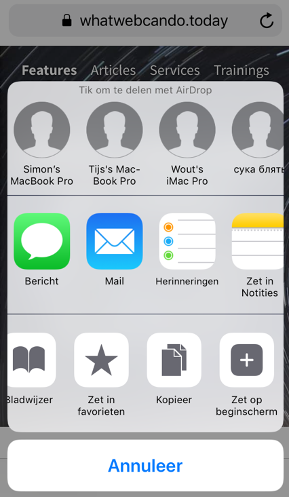
\includegraphics[width=35mm]{./img/installation_ios.png}
		\caption{Screenshot van het installatieproces op een IPhone met IOS 13}
	\end{figure}
	
	\begin{figure}[H]
		\centering
		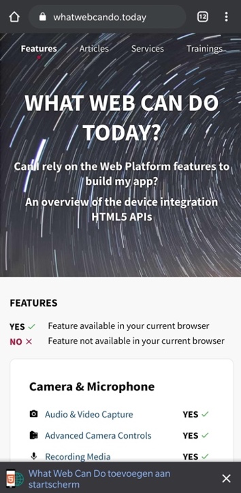
\includegraphics[width=35mm]{./img/installation_android.png}
		\caption{screenshot van het installatieproces op Android 10}
	\end{figure}


	De integratie van de ingebouwde slimme assistent is op IOS beperkter dan op Android. Als een applicatie geïnstalleerd is op een Android toestel, kan Google assistant deze openen aan de hand van een stemcommando. Siri heeft deze functionaliteit niet.
	\autocite{Lathiya2020}
	
	\subparagraph{conclusie}
	
		Er kan geconcludeerd worden dat Android meer open staat voor intergraties met PWA's dan IOS. In deze trend lijkt er niet direct verandering te komen. Google, de ontwikkelaar van Android, is vaak de eerste om nieuwe web API's te ondersteunen.
		
		Langs de andere kant is IOS vaak het laatste besturingssyteem die ondersteuning zal aanbieden voor een web API.


\subsubsection{Desktop besturingssystemen}
	Bij deze vergelijking zullen enkel Windows en Mac OS in beschouwing genomen worden. Andere besturingssysteem hebben relatief gezien niet veel gebruikers. 88,14\% van de computers werkt op Windows en 9,42\% werkt op Mac OS. Slechts 2,44\% van de computers maakt gebruik van andere besturingssystemen.
	\autocite{netMarketShare2020}
	
	Microsoft wil PWA's zo goed mogelijk ondersteunen. Ze zijn zelf ook PWA's aan het ontwikkelen. Een voorbeeld hiervan is Outlook, de populaire online email-client kan nu ook geïnstalleerd worden als PWA.
	\autocite{Microsoft2020a}
	
	PWA's kunnen ook zonder aanpassingen in de Windows store geplaatst worden. Deze applicatie kan dan door alle Windows-toestellen gedownload worden. Er zijn verschillende toestellen die gebruik maken van deze store:
	\begin{itemize}
		\item	Windows 10 toestellen
		\item	Windows S toestellen
		\item	XBox
		\item	Microsoft Hololens 
	\end{itemize}
	
	Windows gaat nog een stap verder dan dit. Het gaat zelf op zoek naar PWA's op het internet en zal deze automatisch toevoegen aan de Windows store. Dit kan wel tegengegaan worden als de uitgever van de PWA dit niet wil.
	\autocite{Gustafson2017} \autocite{Gustafson2017a}
	
	Als een PWA geïnstalleerd wordt op Windows zal deze zich gedragen als een volwaardig programma. De PWA zal opgestart worden in zijn eigen venster. De applicatie kan ook gevonden worden met een zoekopdracht vanuit het startmenu. De applicatie kan ook toegevoegd worden aan de taakbalk en aan het bureaublad.
	
	\begin{figure}[H]
		\centering
		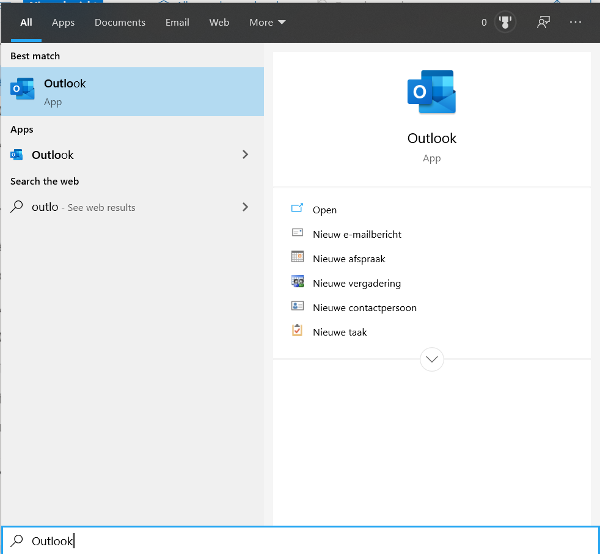
\includegraphics[width=75mm]{./img/Outlook_search_windows.png}
		\caption{screenshot van de zoekresultaten van “Outlook” op Windows 10}
	\end{figure}
	
	
	De tool PWABuilder die gebruikt kan worden om een PWA in de populaire mobiele app-stores te krijgen, is ook ontwikkeld door Microsoft.
	\autocite{PWAbuilder2020}
	
	Microsoft heeft ook een uitgebreide documentatie die ontwikkelaars helpen bij het ontwikkelen van PWA's.
	\autocite{Microsoft2020b}
	
	
	Apple biedt weinig ondersteuning voor PWA's in zijn mobiele besturingssystemen. Deze trend zet zich door op de besturingssystemen voor desktops. In de standaardbrowser, Safari, van de toestellen kan een PWA niet geïnstalleerd worden. Als de gebruiker Google Chrome gebruikt, kan een PWA wel geïnstalleerd worden. Als deze geïnstalleerd is, kan de applicatie ook gevonden worden in een “spotlight search”. De applicatie kan ook vastgemaakt worden aan het dock.
	
	\begin{figure}[H]
		\centering
		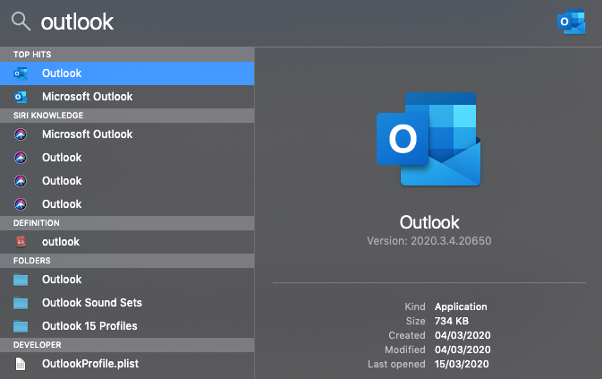
\includegraphics[width=75mm]{./img/Outlook_search_mac.png}
		\caption{screenshot van de zoekresultaten van “Outlook” op Mac Os}
	\end{figure}
	
	Deze algemene trend waarbij Apple PWA's bewust niet ondersteunt, lijkt niet snel te veranderen. John Wilander, een ontwikkelaar binnen Apple, bekritiseerde openlijk PWA's als een technologie die van Google is en dat dit niet in de planning zit van Apple. 
	\autocite{Wilander2019}
	
	
	\subparagraph{Conclusie}
	Er kan geconcludeerd worden dat Windows en Mac OS een volledig andere filosofie hebben als het aankomt op PWA's. 
	
	Windows probeert een zo goed mogelijke ondersteuning te geven aan PWA's. PWA's worden binnen windows behandeld als een volwaardig programma. Als een PWA geïnstalleerd is, is het moeilijk te onderscheiden van een ander native programma.
	PWA's zijn binnen windows ook eenvoudig om te installeren.
	Micorosoft probeert ontwikkelaars ook te ondersteunen in het ontwikkelen van PWA's, dit doen ze door een uitgebreide documentatie en tools aan te bieden.
	
	Apple daarintegen is meer gesloten ten opzichte van PWA's. Vanuit de standaard browser kunnen er helemaal geen PWA's geïnstalleerd worden. Via google Chrome is dit wel mogelijk.
	